\section{Latency in WAN}
\label{sec:latency-wan}

\subsection{Methodology}
\label{sec:methodology}


We derive our measurement methodology from King \cite{gummadi2002king} and Turbo-King \cite{leonard2008turbo}, and developed a Turbo-King variant illustrated in Fig.\,\ref{fig:king_model}. The King method leverages DNS name-servers to make measurements that approximate latency between arbitrary end hosts. It utilizes properties of DNS to coerce recursive DNS resolvers into making outbound queries on behalf of measuring party. Turbo-King builds upon King by allowing for detection of DNS forwarders. DNS forwarders aggregate DNS queries within a network that target external DNS servers and can serve responses. The original King method has no means of detecting these servers, and as a result they may skew measurement results.

\subsubsection{Overview}
Our methodology is composed of 4 elements, a measurement node, a central domain name server, and 2 target name servers. A measurement nodes is composed of a DNS client and server. A node accepts remote-procedure calls that specify 2 target DNS servers and returns both DNS latency measurements and multiple round trip time calculations to the first target server. The central domain name server simply refers incoming DNS requests to the originating measurement node. The 2 target name servers must have known locations and the first must be an open-recursive resolver. Below we outline the measurement process.

\begin{enumerate}
	\item DNS Client on measurement node will issue a request to the first target DNS server. The requested URL will be of the form "qid.myAddr.mydomain.com", where qid is the query id, myAddr is an encoding of the measurement nodes public name, and mydomain is the domain controlled our central name server.
	\item The target server will issue a request containing the requested URL to the central name server
	\item The central name server will decode the "myAddr" element of the requested URL to the url of the originating measurement node. It will return a response to the querying target server with a referral to the measurement node.
	\item The target name server will then issue a DNS query with the requested URL to the measurement node.
	\item The measurement node will receive a DNS query, lookup the query id and return a referral with the corresponding second target DNS server.
	\item The first target DNS server will issue a request to the second DNS server
	\item The second server will deliver a response (to be discussed more)
	\item The first target name server will then pass along this response to the DNS client of the measurement node.
\end{enumerate}

We record the time delta between step 5 and 8, and subtract the round-trip time between the measurement node and the first target to generate a latency measurement between the two target DNS servers.

\subsubsection{Round Trip Time Latency}
To determine the round trip latency between a measurement node and the first target server, we issue a DNS query for a random subdomain in the domain controlled by the target name server. We issue this request multiple times to allow and discard the first measurement. In this way we allow for the request to be cached on the target server and minimize the processing time to generate more accurate round-trip time measurements. We adopted This method is over ICMP ping because a fraction of DNS servers we queried did not respond to ICMP requests.

\subsubsection{Additional Considerations}
It is important to note that upon the first DNS request to the second target DNS server, that server itself may try a complete resolution if it is an open resolver. In this case, the second target server will issue a request to resolve our domain and will be referred to the originating measurement node. It will issue a request to this node that contains the original query id; in this event the measurement node will not issue a response and allow the second target server to time out. The second target will then return a NXDomain response to the first target name server, and upon subsequent requests for our domain (within some time period dictated by that servers caching policy) it will issue continue to issue error responses. Thus, we always discard the first latency measurement in every round to account for this additional lookup latency.

\begin{figure}
  \centering
  \includegraphics[width=\linewidth]{../figs/king_model.pdf}
  \vspace{-1em}
  \caption{King/T-King method illustration}
  \label{fig:king_model}
\end{figure}

\subsubsection{Reverse DNS Crawl}
The Turbo-King methodology requires a large set of known open recursive name servers to generate latency measurements. An open recursive name server will respond to requests for any arbitrary domain from clients outside its AS. Only the first target name server must be an open resolver, the second server may be any DNS server that issues any response to external queries. To build a set of DNS servers, we performed a crawl of the reverse DNS tree.

Reverse DNS requests take the form of requests for the ".in-addr.arpa" prefixed in reverse order with the octets of the IP to be resolved. Queries operate as normal DNS queries do, where in each octet is a sub-domain for which a DNS server is responsible for.
At the first level of the DNS tree we issue a query to the "in-addr.arpa" domain for the first octet (1-255) and receive responses (start of authority, SOA, records) that indicate the servers responsible for the next level of the tree. We continue by issuing requests for the second octet (second.first.in-addr.arpa) to these servers, and we proceed similarly for the third octet. If we do not receive an SOA record skip further search down the tree that contains that prefix. At each step, we record any responses that indicate authoritative name servers. Thus, after a three level traversal we are left with a set of authoritative DNS servers. We implemented and deployed a multi-threaded crawler to Amazon EC2 that was able to complete a traversal on the order of 1 day.

\subsubsection{Open Resolvers}
Our methodology requires that the first DNS resolver be an open recursive resolver. To build this set, we leverage the service provided by the DNS Measurement Factory. By issuing a DNS query to the Measurement Factory name server it will check if that server is an open resolver and return the results.\cite{dnsfactory}

\begin{figure}
  \centering
  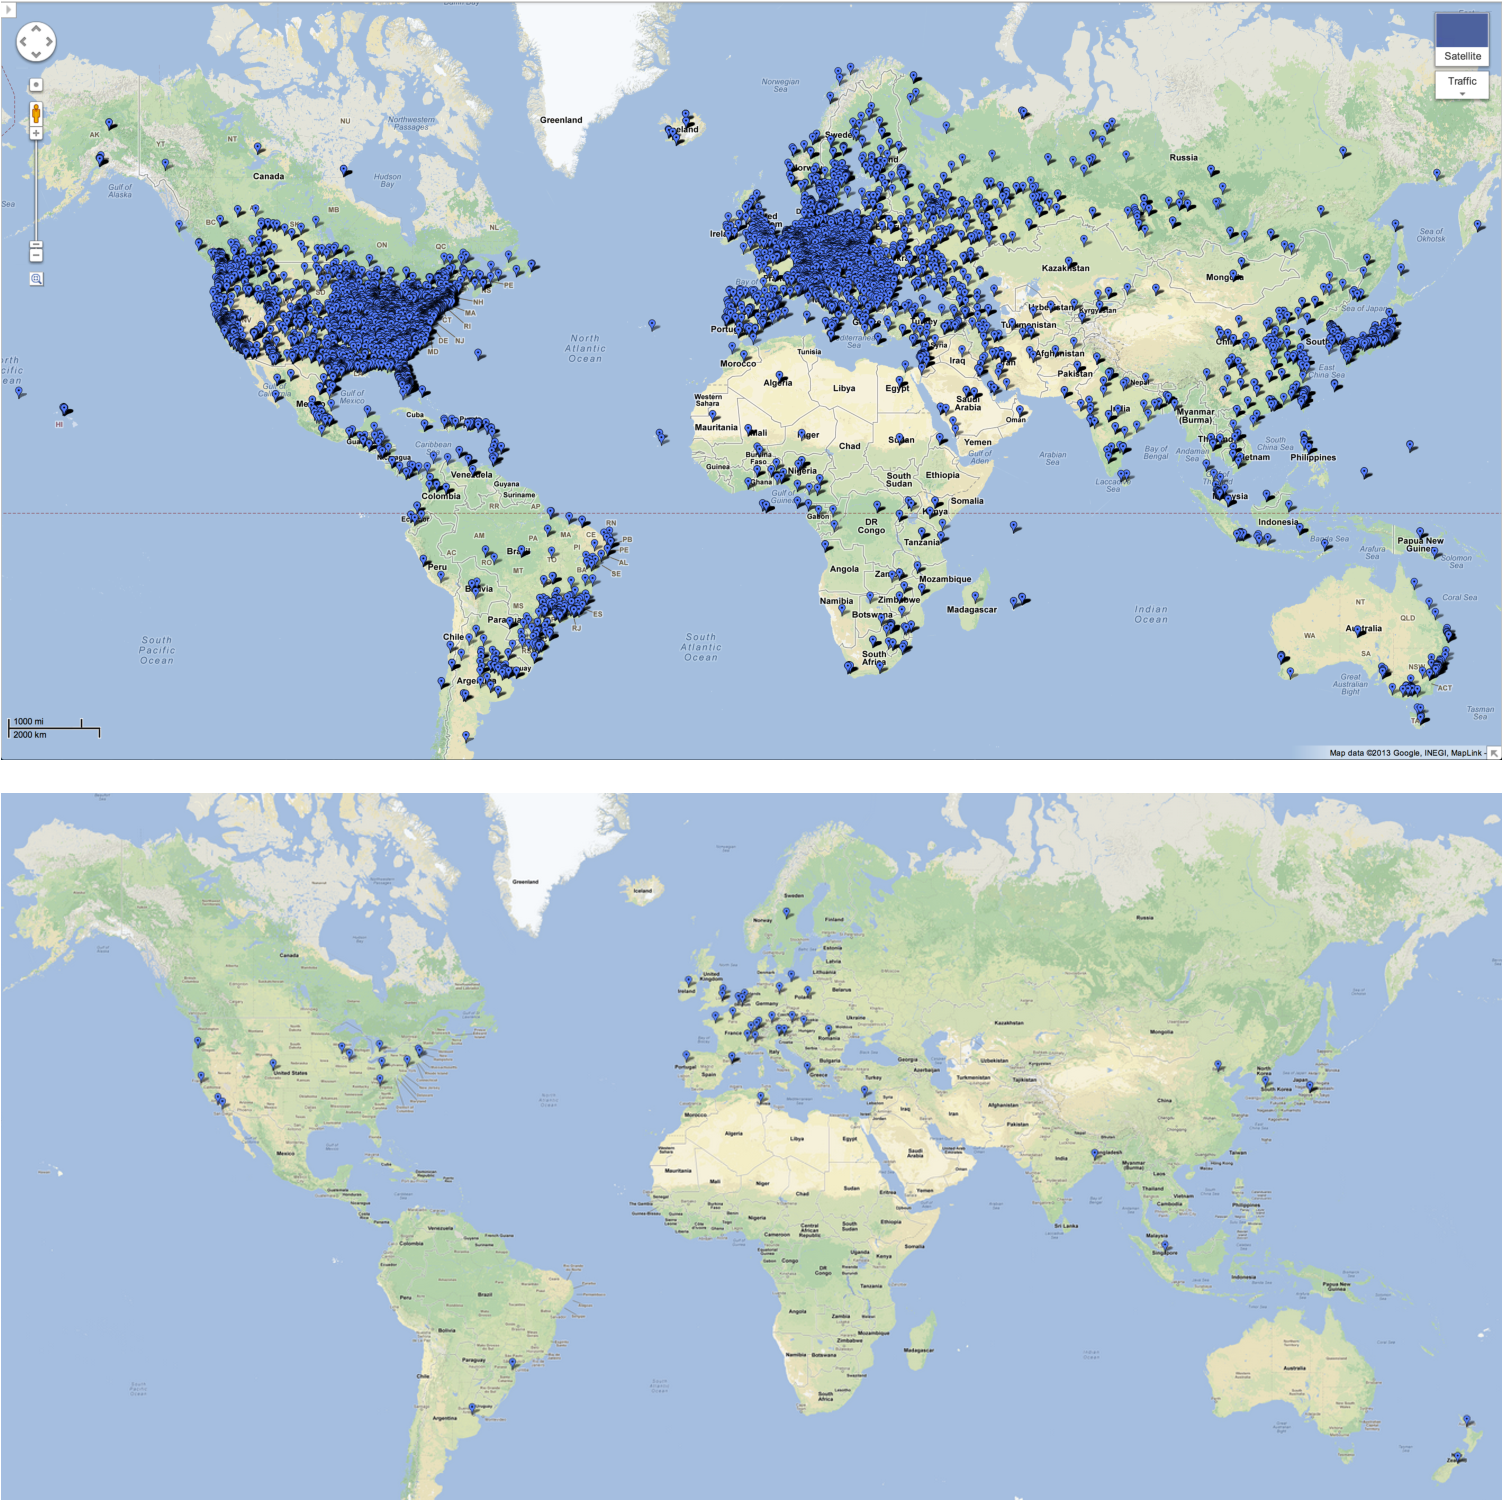
\includegraphics[width=\linewidth]{../figs/geo_viz.pdf}
  \vspace{-1em}
  \caption{(Top) Distribution of open resolvers, visualized using Google Map, (Bottom) Distribution of PlanetLab nodes that we are using, visualized using Google Map}
  \label{fig:geo_viz}
\end{figure}


\subsection{Implementation and Experiment}
\label{sec:impl-exper}

Using a combination of EC2 and Planet Lab servers, we collected approximately x.xx successful measurement results between 4/20/13 and 5/4/13.

\subsubsection{Measurement Node}
We utilized the dnspython libraries to implement our Turbo-King variant. Each measurement node runs a Turbo-King server (composed of a DNS client and server) which exposes a remote procedure call service using the RPYC library. We deployed the Turbo-King server to 56 Planet Lab nodes (Fig. X).

\subsubsection{Central Name Server}
Our central name server is implemented using the Python twisted framework, which allowed for highly parallel and asynchronous handling of DNS queries. We deployed 2 name-servers on Amazon EC2.

\subsubsection{Controller}
Latency measurements were centrally managed from a controller running on EC2. The controller is responsible for issuing remote-procedure calls to Turbo-King servers and storing the resulting data. The controller randomly selects 2 target name servers, the first from the set of open recursive resolvers, and the second from the set of all resolvers. It then determines the 10 nearest Turbo-King servers to the first target, issues a remote procedure call to each, and stores the results in a relational database. The controller is composed of multiple threads that follow this procedure and run continuously.

\subsection{Analysis}
\label{sec:analysis}

\subsubsection{Distribution of Distances}

\begin{figure}[!tbh]
  \centering
  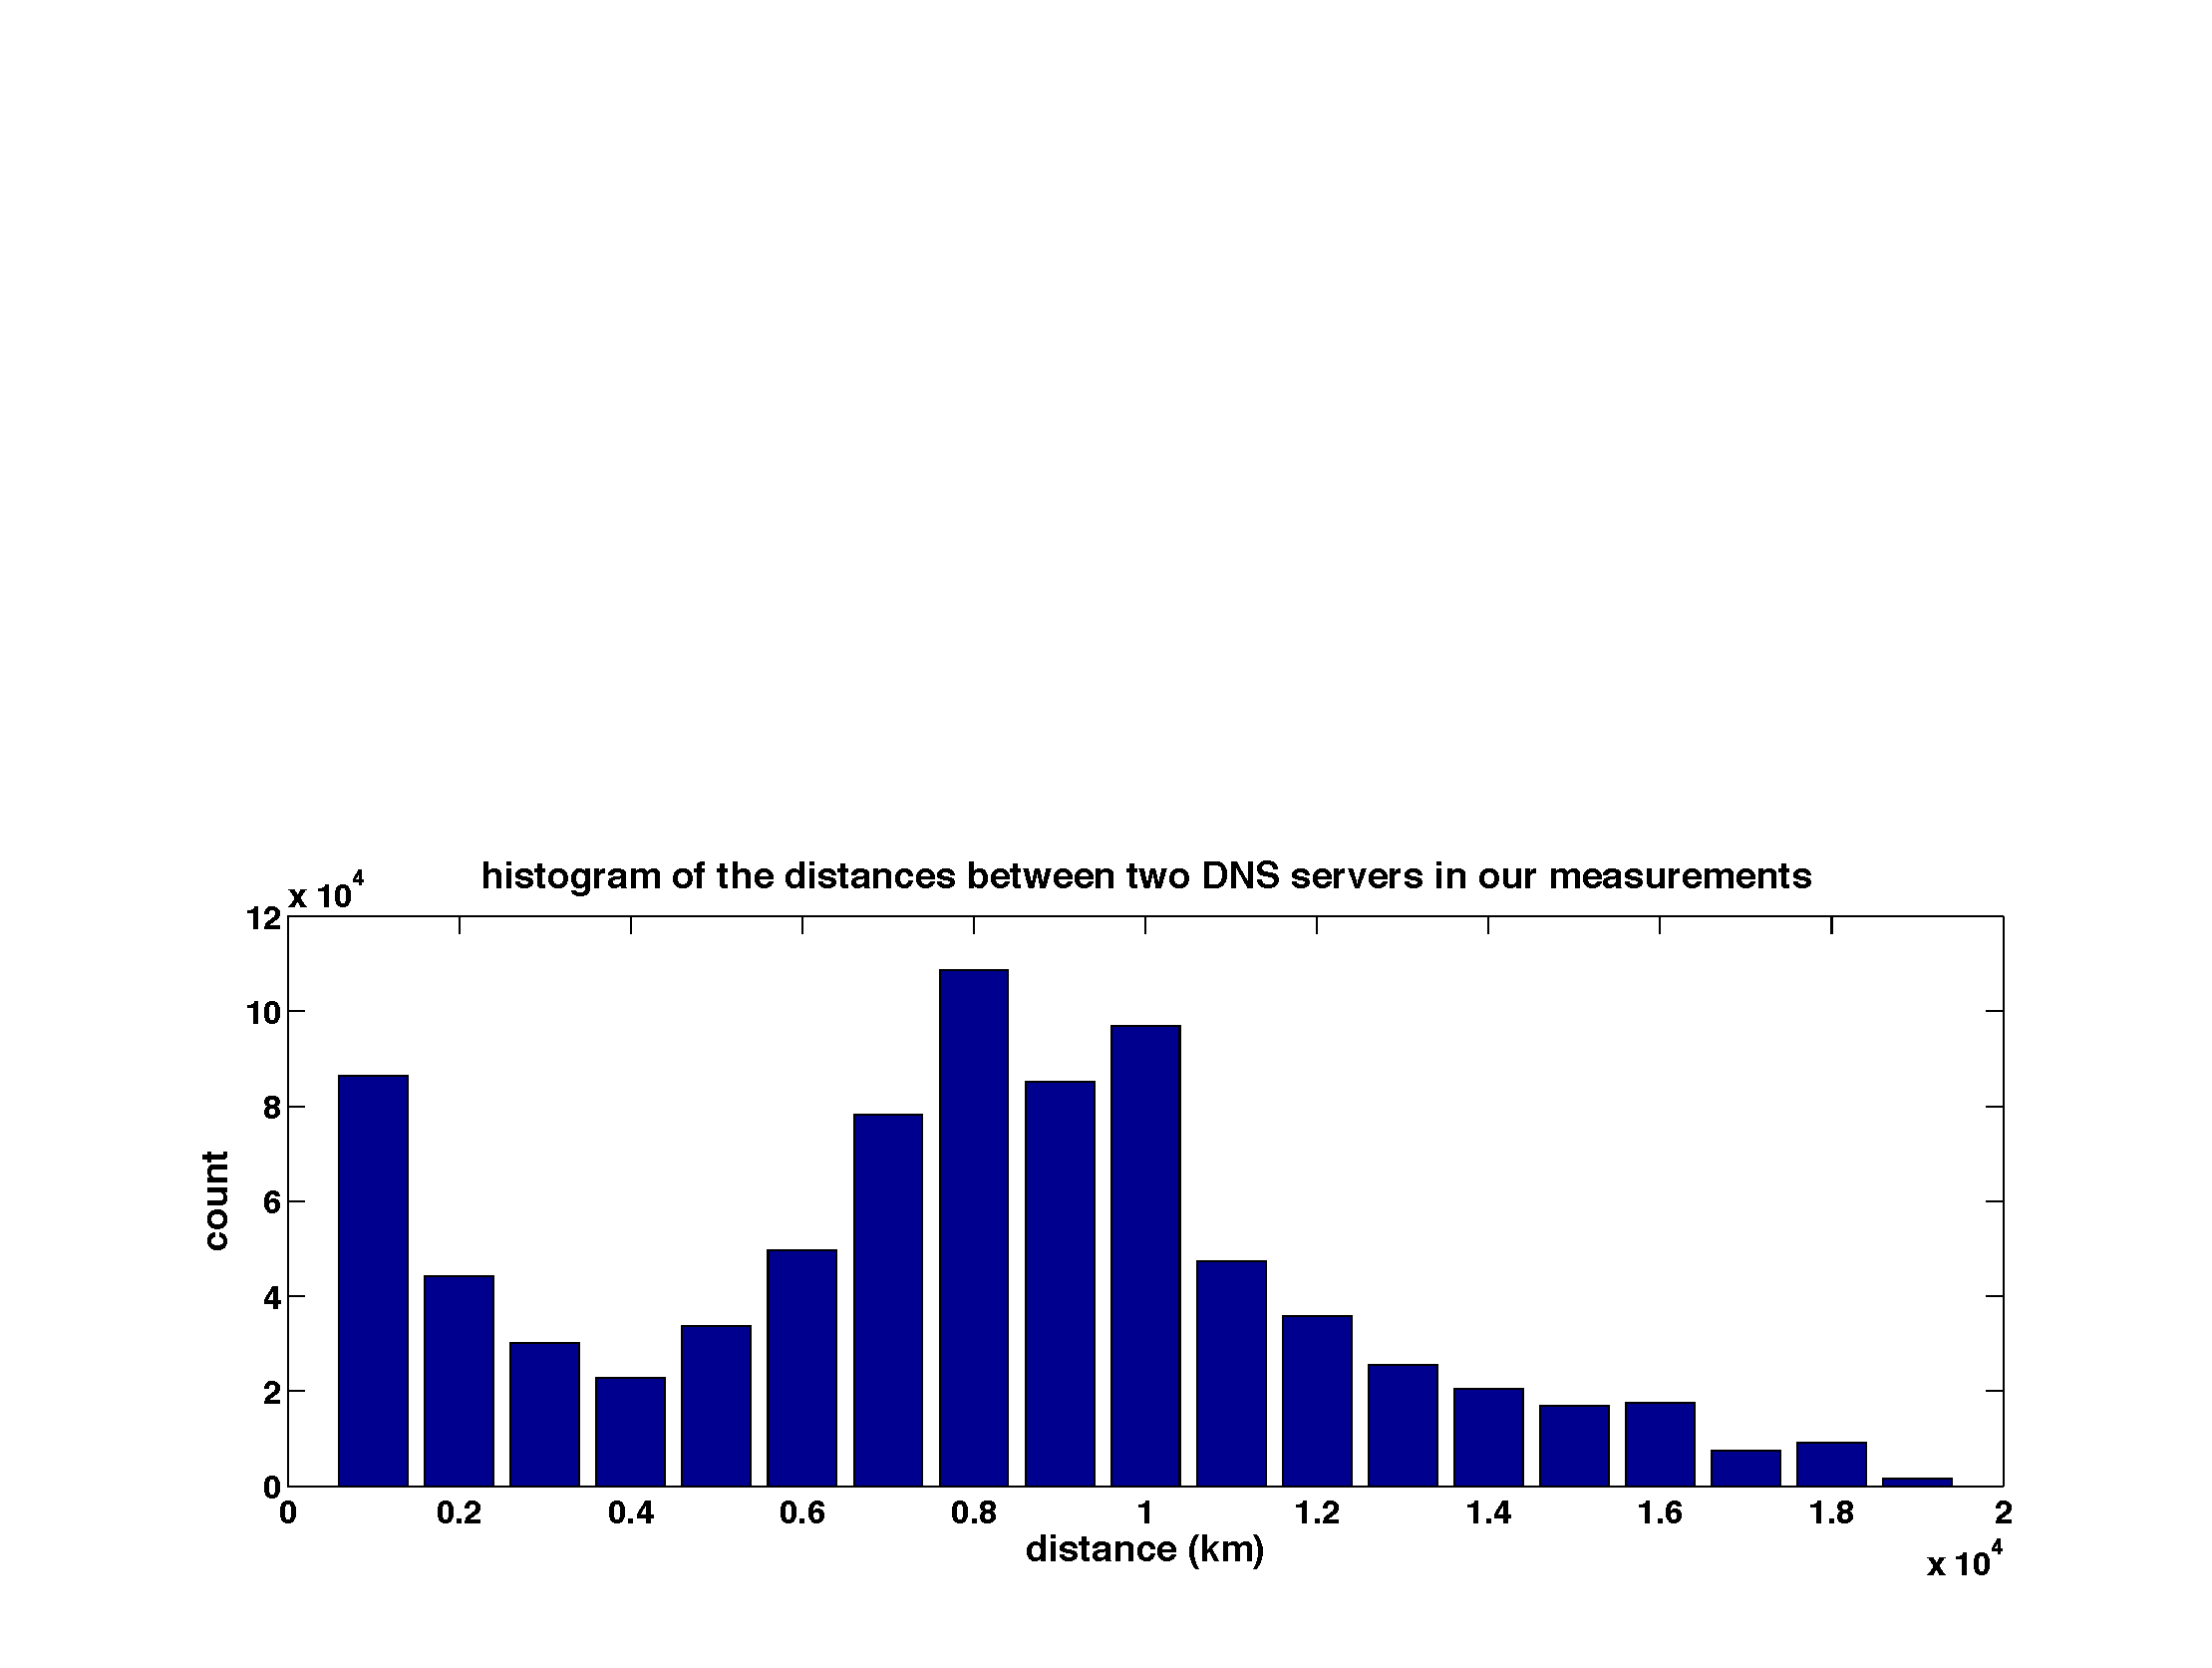
\includegraphics[width=\linewidth]{../figs/King_distance_distrbution.pdf}
  \vspace{-1em}
  \caption{Distribution of distances of measured latencies}
  \label{fig:latency_distance_distribution}
\end{figure}

Figure\,\ref{fig:latency_distance_distribution} represents the distribution of distances between target DNS servers in the collected measurements. It is interesting to note that the distribution is bimodal (peaking at 1000 km and 8000 km). We believe this property is reflective of the inter and intra continental patterns in our DNS resolver set (fig.\,\ref{fig:geo_viz}). Resolvers are concentrated in USA and Europe, and as such we believe the high probability of randomly selecting a USA to USA or Europe to Europe target pair generates the first peak of the measurement distribution. Similarly, the second peak is generated by a USA to Europe (or vice versa) target pair.

\subsubsection{Filtering Measurements}
In this section we outline the parameters used to filter our collected measurements before performing analysis. We will briefly discuss the impact on the dataset and rationale for using these parameters.

\begin{table}[!htb]
  \begin{tabular}{p{2.3cm} | p{.6cm} | p{4.6cm}}
    \hline
    Filter & \% & Description \\
    \hline
    Faster than 2/3 the speed of light & 1.8\% & These measurements can be attributed to incorrect GeoIP resolution of target servers. \\
	\hline
	Negative Latency & 0.8\% & Still analyzing \\
	\hline
	High Latencies & 4.8\% & 5 second timeout on results \\
	\hline
	Forwarder Responses & 23\% & Forwarders can have small or large impact on results depending on location relative to target server (Fig.\,\ref{fig:forwarder_viz}) \\
	\hline
	Zero Distance & 0.4\% & GeoIP inaccuracy, especially for DNS servers within the same AS \\
	\hline
	First Result of DNS Query to new server & 48.5\% & Discussed above, large size is reflective of issues with controller and PlanetLab node response rate, not methodology. \\
    \hline
  \end{tabular}
  \vspace{1em}
  \caption{Filtering Parameters, percent of dataset, and description}
  \label{tab:filter}
\end{table}

\subsubsection{Latency vs. Distance}
We performed our analysis by grouping measurements into 1000 km buckets and plotting the average latency (Fig.\,\ref{fig:latency_dist}). The blue error bar represents 5 - 95 percentiles in each bucket. It can be observed from the graph that, in general, latency does in fact grow with distance. The fit line in Fig.\,\ref{fig:fit_curve} shows that the relationship between latency and distance can be approximated with an increasing linear function.

\begin{figure*}
  \centering
  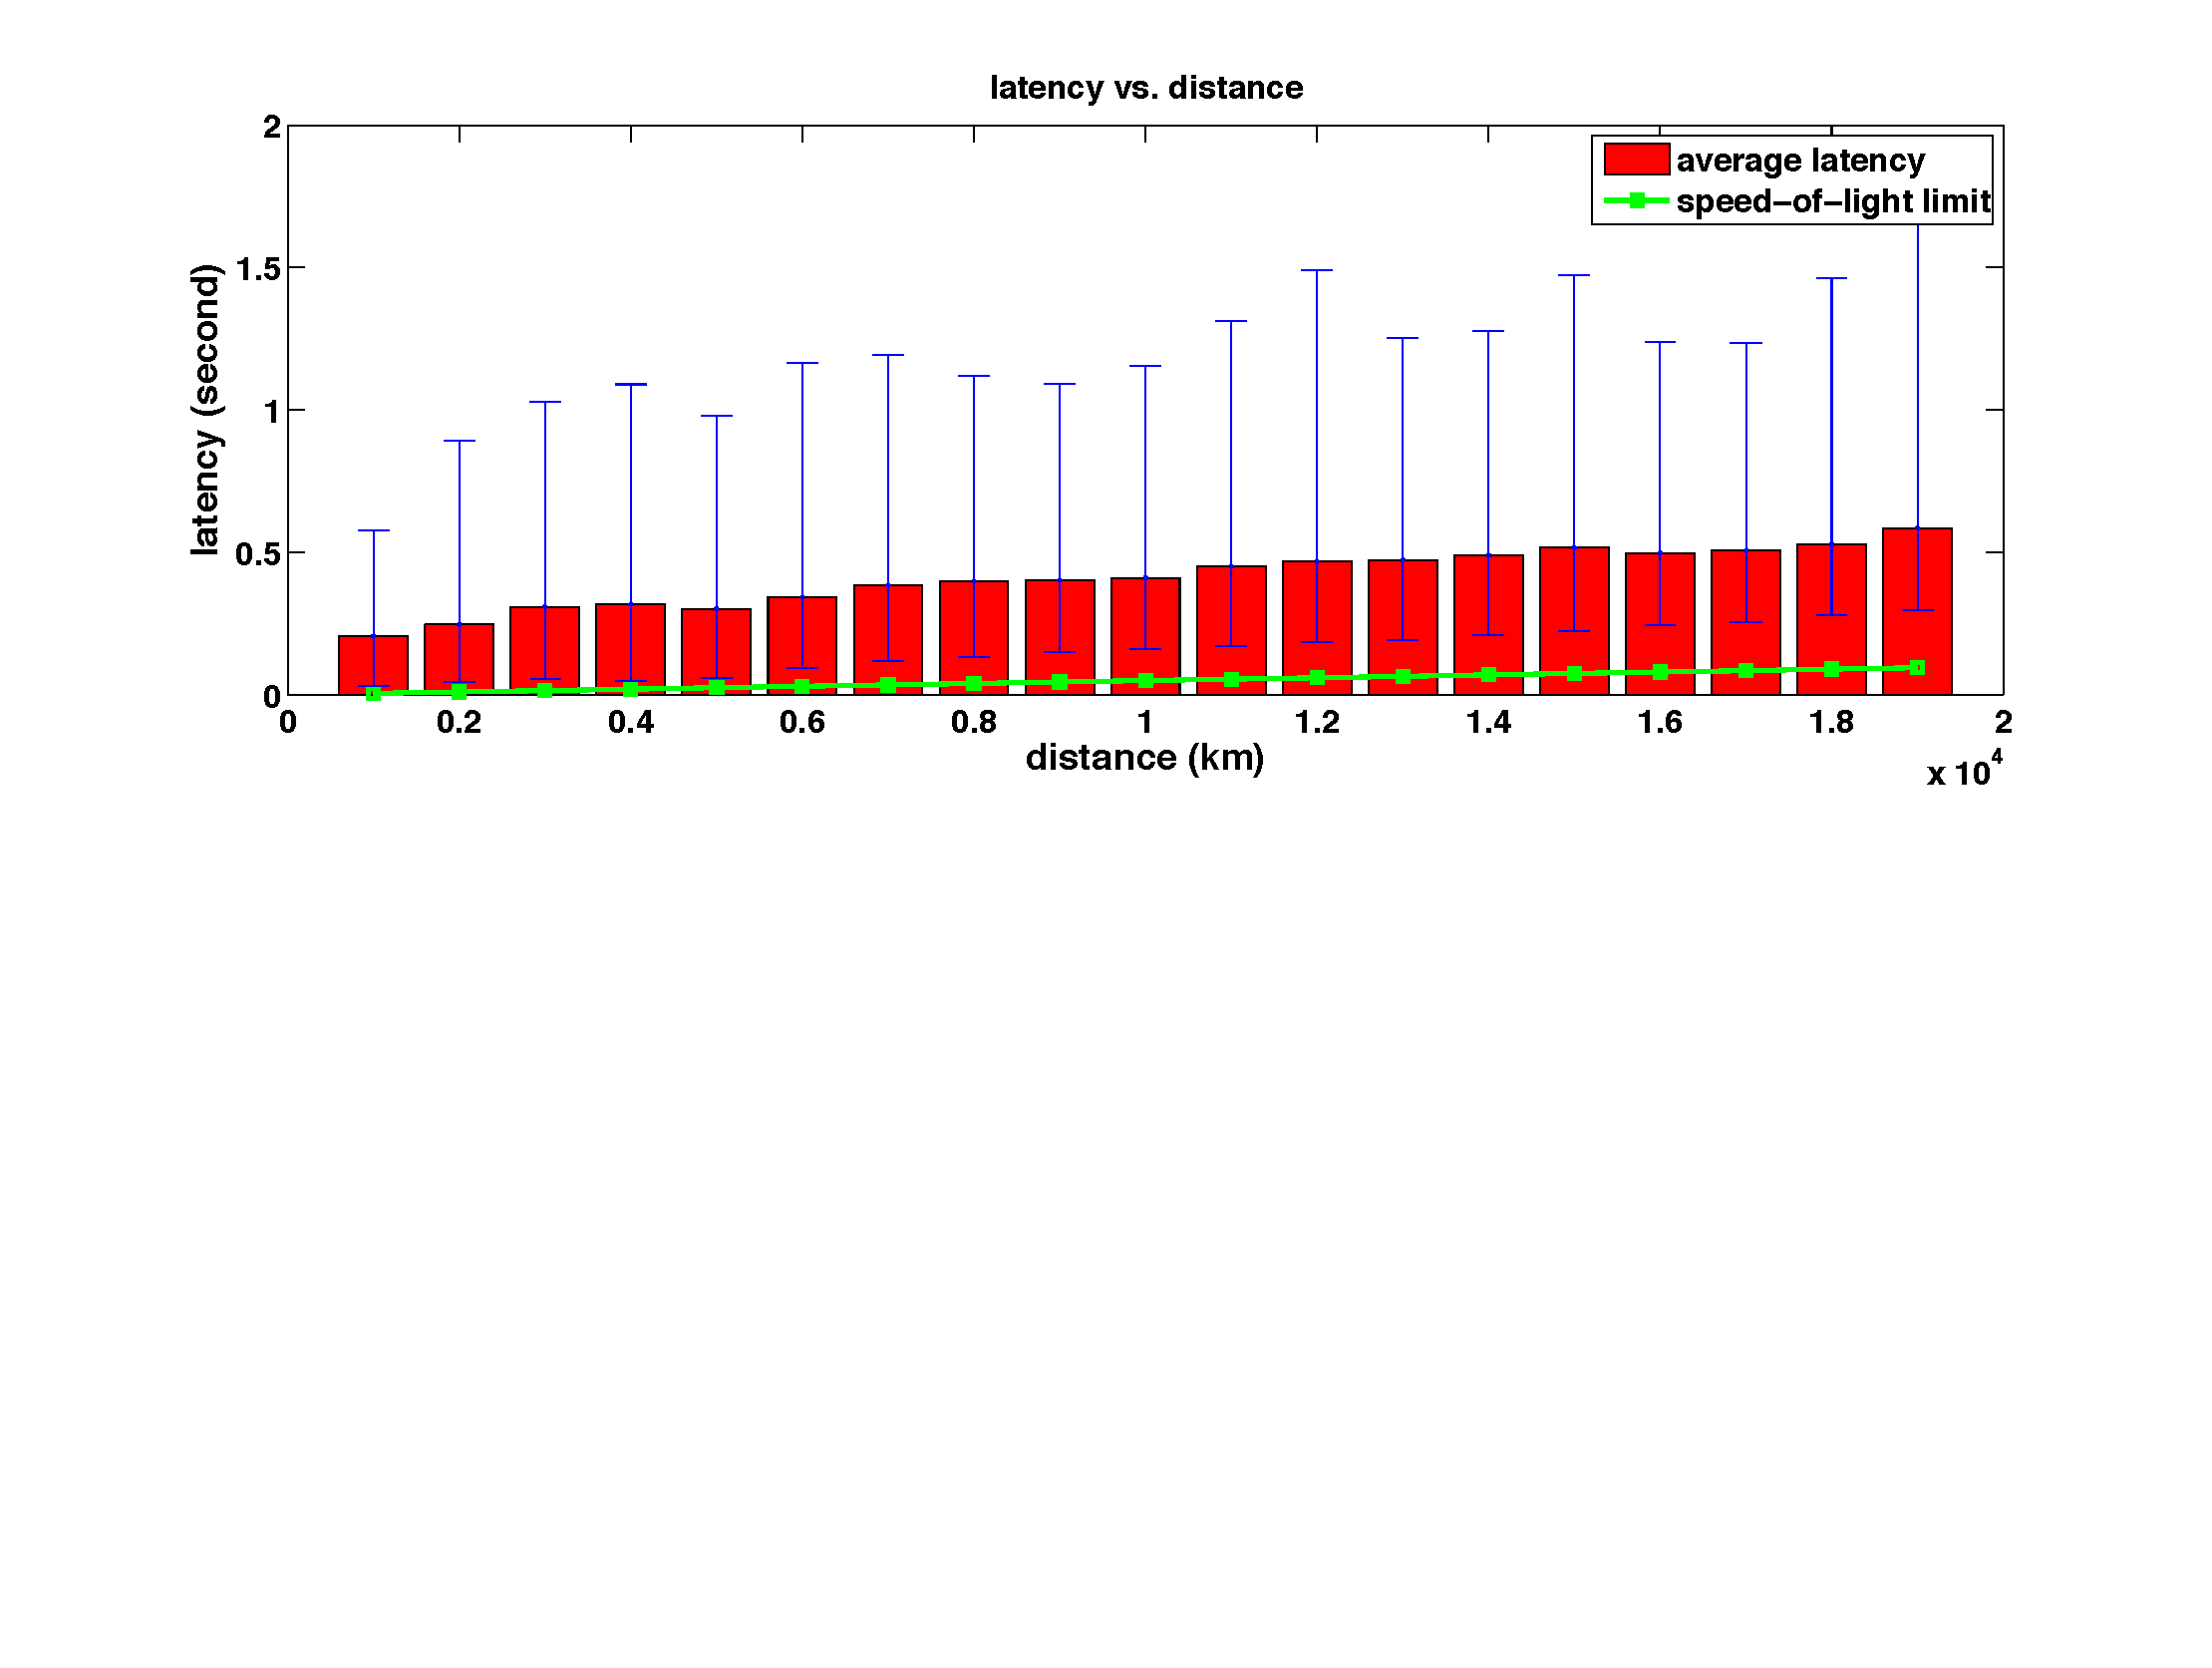
\includegraphics[width=\linewidth]{../figs/King_latency_dist.pdf}
  \vspace{-1em}
  \caption{Latency vs. Distance}
  \label{fig:latency_dist}
\end{figure*}

\begin{figure}
  \centering
  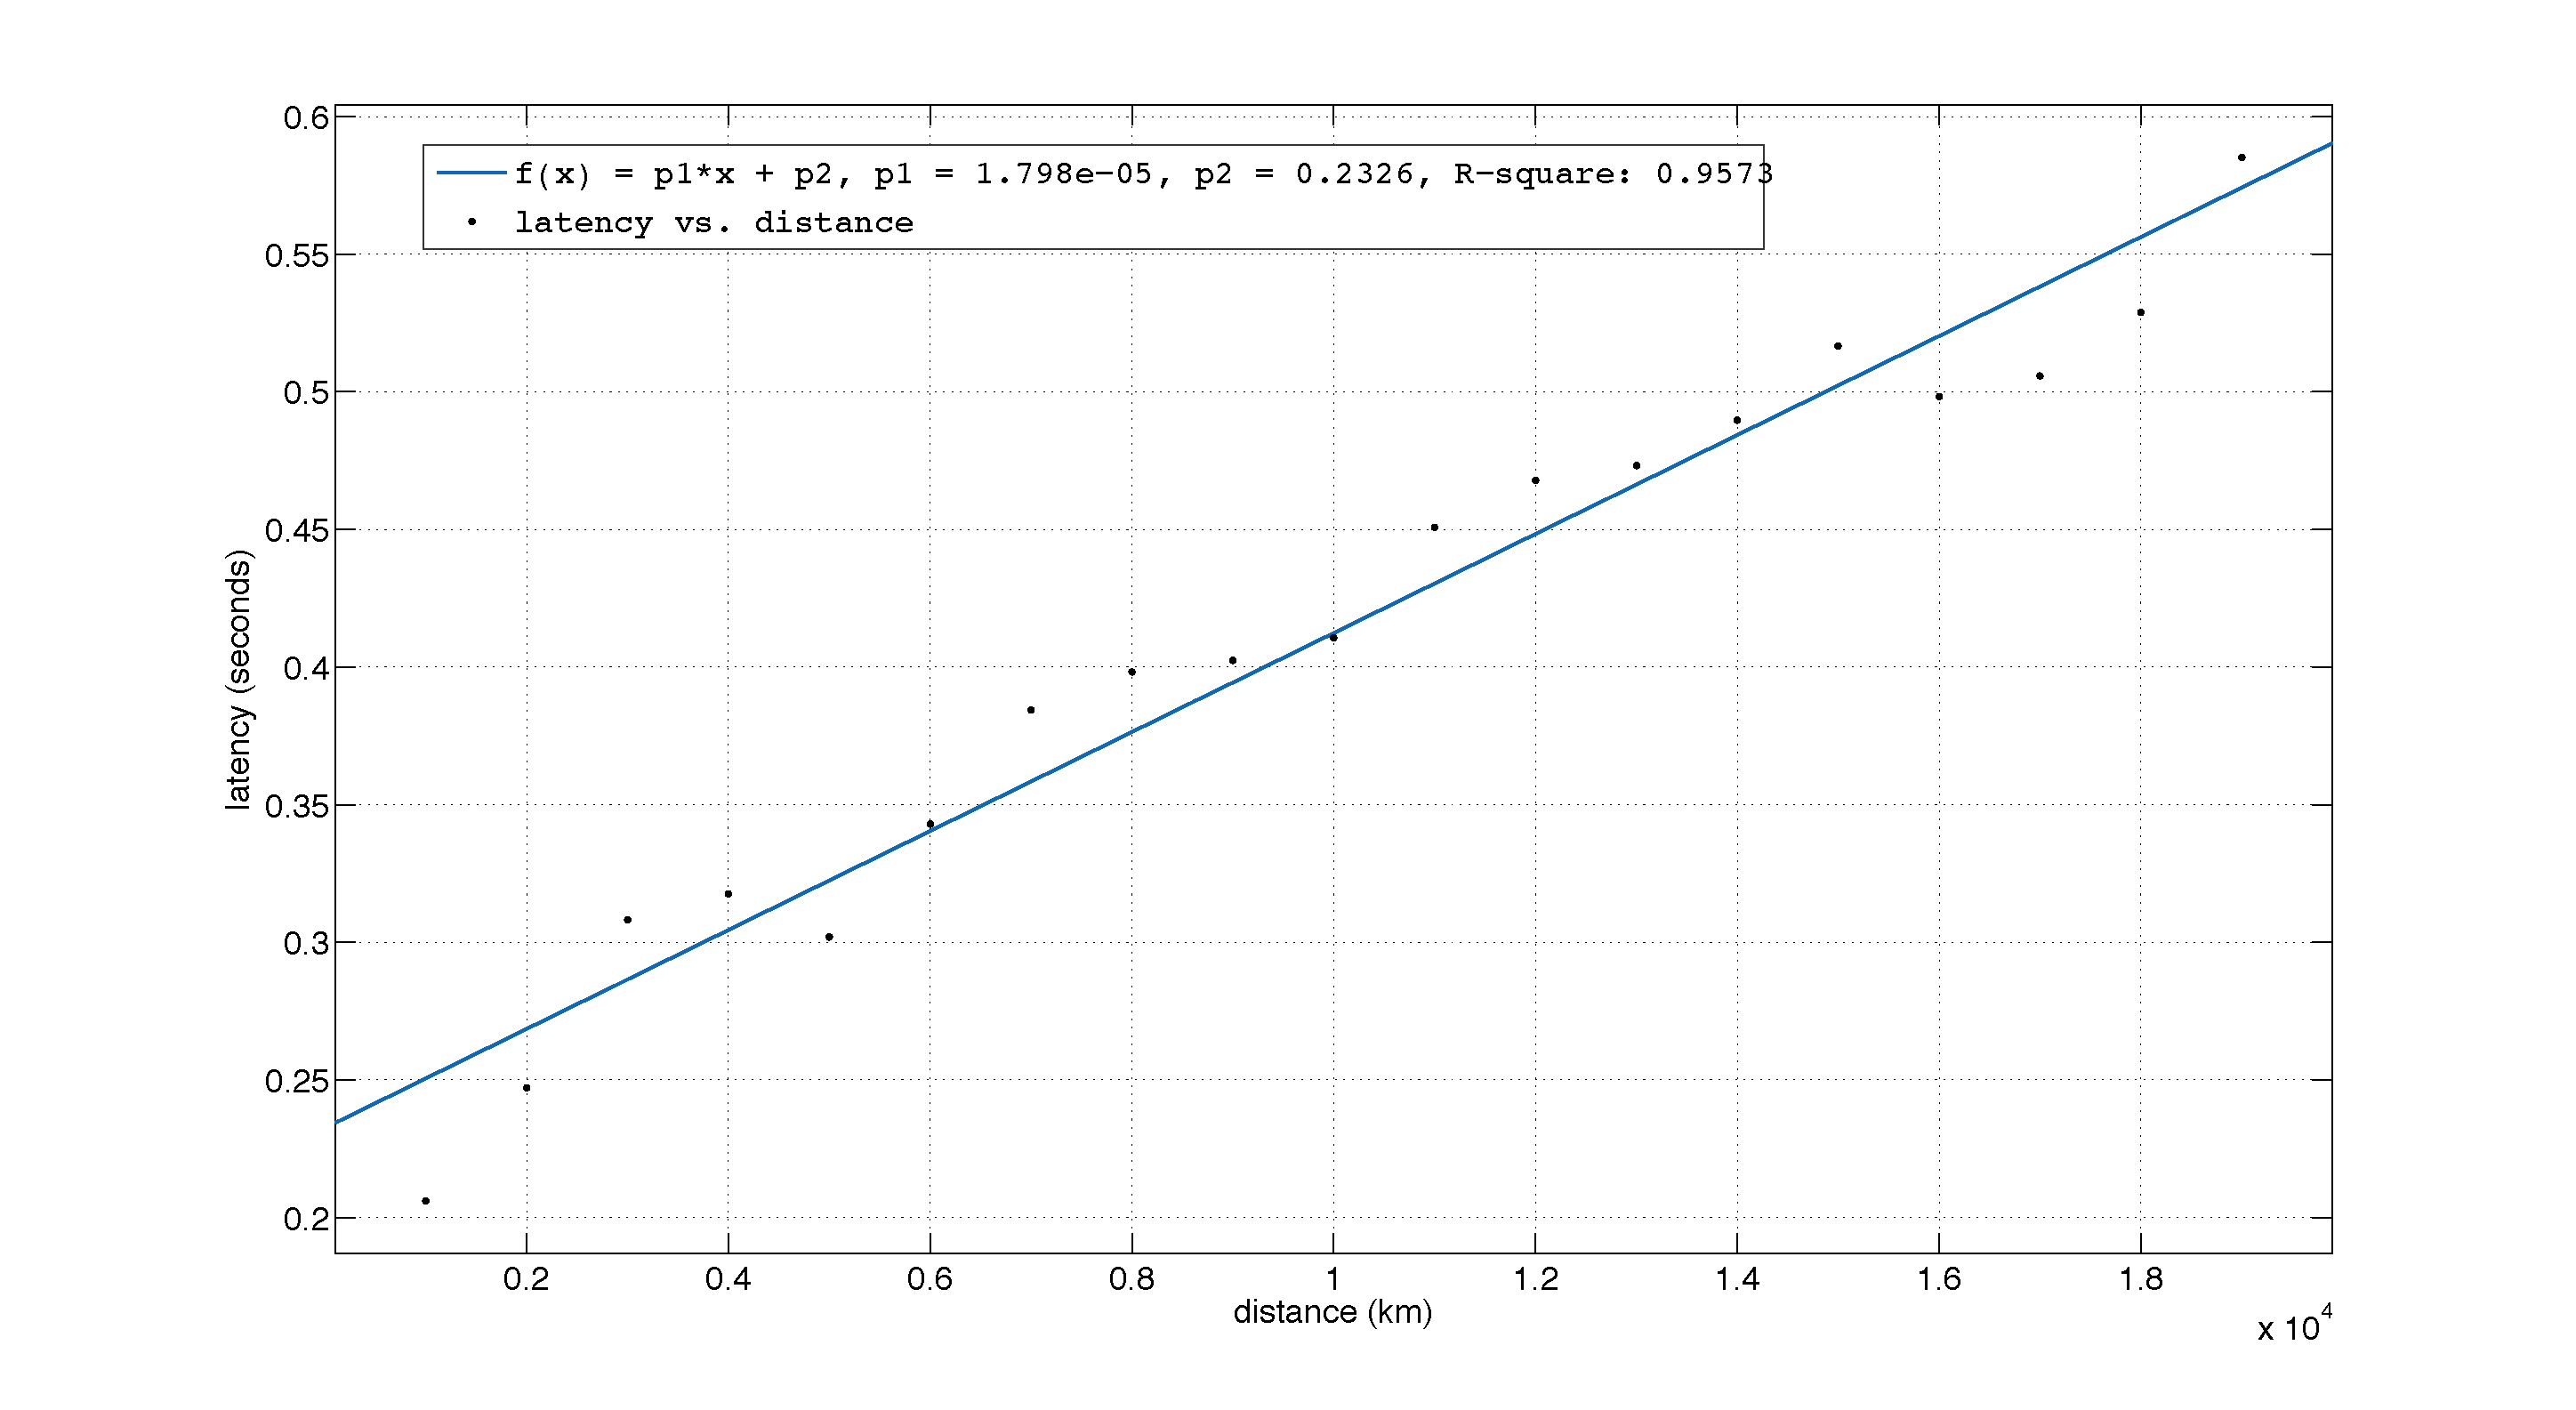
\includegraphics[width=\linewidth]{../figs/fit_curve.pdf}
  \vspace{-1em}
  \caption{Linear fitting of latency vs. distance}
  \label{fig:fit_curve}
\end{figure}

\begin{figure}[t]
  \centering
  \includegraphics[width=\linewidth]{../figs/dns_forwarder.pdf}
  \vspace{-1em}
  \caption{A selected sample of DNS forwarders in our measurement set, where each path represents the distance between forwarder and target server}
  \label{fig:forwarder_viz}
\end{figure}

%%% Local Variables: 
%%% mode: latex
%%% TeX-master: "main"
%%% End: 
